%!TEX program = xelatex
\documentclass[a4paper,UTF8]{ctexart}
\usepackage[unicode=true,colorlinks,urlcolor=blue,linkcolor=blue,bookmarksnumbered=true]{hyperref}
\usepackage{latexsym,amssymb,amsmath,amsbsy,amsopn,amstext,amsthm,amsxtra,color,multicol,bm,calc,ifpdf}
\usepackage{graphicx}
\usepackage{diagbox}   % 绘制表格斜线
\usepackage{enumerate}
\usepackage{epstopdf}
\usepackage{fancyhdr}
\usepackage{subfigure}
\usepackage{listings}
\usepackage{multirow}
\usepackage{makeidx}
\usepackage{xcolor} 
\usepackage{algorithm}    % format of the algorithm
\usepackage{algorithmic}    % format of the algorithm
\usepackage{fontspec}                            % 建立索引宏包
\graphicspath{{figures/}}  % 设置图片搜索路径
\theoremstyle{plain} \newtheorem{theorem}{定理}[section]
\theoremstyle{plain} \newtheorem{definition}{定义}[section]
\theoremstyle{plain} \newtheorem{lemma}{引理}[section]
\theoremstyle{plain} \newtheorem{proposition}{命题}[section]
\theoremstyle{plain} \newtheorem{example}{例}[section]
\theoremstyle{plain} \newtheorem{remark}{注}[section]
\theoremstyle{plain} \newtheorem{corollary}{推论}[section]
\newfontfamily\courier{Courier New}
\lstset{linewidth=1.1\textwidth,
        numbers=left, %设置行号位置 
        basicstyle=\small\courier,
        numberstyle=\tiny\courier, %设置行号大小  
        keywordstyle=\color{blue}\courier, %设置关键字颜色  
        %identifierstyle=\bf,
        commentstyle=\it\color[cmyk]{1,0,1,0}\courier, %设置注释颜色 
        stringstyle=\it\color[RGB]{128,0,0}\courier,
        %framexleftmargin=10mm,
        frame=single, %设置边框格式  
        backgroundcolor=\color[RGB]{245,245,244},
        %escapeinside=``, %逃逸字符(1左面的键),用于显示中文  
        breaklines, %自动折行  
        extendedchars=false, %解决代码跨页时,章节标题,页眉等汉字不显示的问题  
        xleftmargin=2em,xrightmargin=2em, aboveskip=1em, %设置边距  
        tabsize=4, %设置tab空格数  
        showspaces=false %不显示空格  
        basicstyle=\small\courier
       }  
\newenvironment{mysolution}{{\color{blue} 解}: }{{\color{magenta}\qed}}
\newcommand\diff{\,{\mathrm d}} %定义微分d
\newcommand{\p}[3]{\frac{\partial^{#1}#2}{\partial{#3}^{#1}}}  %定义求偏导算子
\newcommand{\ucite}[1]{\textsuperscript{\cite{#1}}}  %参考文献引用:上标用\ucite{ },文中用\cite{ }

\begin{document}
\title{

\includegraphics[width=0.65\textwidth]{onepiece.pdf}\\
\vspace{2em}
\textbf{模型评价学习笔记}}
\author{\emph{李向阳} \quad {\color{blue} d1142845997@gmail.com} }
\date{}


\maketitle
\thispagestyle{empty}

\newpage


\tableofcontents

\newpage

\section{引入}
我们目前已经介绍了很多机器学习的模型了, 包括分类、聚类、回归等等. 不过, 我们并没有细致的去衡量模型的泛化能力, 这其实是性能度量(performance measure)的问题, 这一次我们来稍微系统的介绍一下.

在预测任务中, 给定训练数据集$D = \{ (\bm{x}_1, y_1), (\bm{x}_2, y_2), \cdots, (\bm{x}_m, y_m) \}$, 其中$y_i$是样本$\bm{x}_i$的真实标记(在分类问题中是离散的, 在回归问题中是连续的). 如果要评价一个模型$f$的性能, 其实就要把模型的预测结果$f(\bm{x})$与真实标记$y$进行比较.


\section{回归任务}
回归模型的评价标准比较简单, 也很容易想到, 既然是预测连续值, 那标准自然是均方误差
\begin{equation}
E(f; D) = \frac{1}{m} \sum_{i=1}^{m} (f(\bm{x}_i) - y_i)^2
\end{equation}

更一般的, 对于数据分布$\mathcal{D}$和概率密度函数$p(\cdot)$, 均方误差可表示为
\begin{equation}
E(f; \mathcal{D}) = \int_{\bm{x} \sim \mathcal{D}} (f(\bm{x}) - y)^2 p(\bm{x}) \diff \bm{x}
\end{equation}


\section{分类任务}
\subsection{准确率和错误率}
模型分类的准确率和错误率恐怕是最常用也最容易想到的了. 简言之, 准确率就是分类正确的样本数占样本总数的比例, 错误率即是分类错误的样本数占样本总数的比例. 如果用式子表示, 对样本数据集$D$, 错误率为
\begin{equation}
E(f; D) = \frac{1}{m} \sum_{i=1}^{m} \mathbb{I}(f(\bm{x}_i) \neq y_i)
\end{equation}

准确率为
\begin{equation}
\mathrm{acc}(f; D) = \frac{1}{m} \sum_{i=1}^{m} \mathbb{I}(f(\bm{x}_i) \neq y_i) = 1 - E(f; D)
\end{equation}


\subsection{查准率和查全率}
准确率和错误率虽然常用, 但是不能满足所有需求. 比如垃圾短信识别, 我们可能也会关心所有垃圾短信中有多少比例被识别了出来. 诸如此类的问题, 就需要引入查准率和查全率等指标. 这些标准主要适用于二分类问题.

二分类问题(通常将关注的类视为正类, 其它类为负类)结果的混淆矩阵(confusion matrix)如下表\ref{confuse}.
\begin{table}[!htb]
\centering
\caption{二分类混淆矩阵}
\label{confuse}
\begin{tabular}{ll|c|c|}
\cline{3-4}
   &    & \multicolumn{2}{c|}{预测值} \\ \cline{3-4} 
   &    & 正例          & 负例         \\ \hline
\multicolumn{1}{|l|}{\multirow{2}{*}{实际值}} & 正例 & TP & FN   \\ \cline{2-4} 
\multicolumn{1}{|l|}{}  & 负例 & FP   & TN   \\ \hline
\end{tabular}
\end{table}

混淆矩阵怎么看? 其实行的标记是真实标记, 列的标记为预测标记. 也就是说, 以上 4 中情况分别表示
\begin{itemize}
\item TP ----- 真正例(True Positive): 本身为正类, 也被预测为正类的样本数

\item FN ----- 假负例(False Negative): 本身为正类, 却被预测为负类的样本数

\item FP ----- 假正例(False Positive): 本身为负类, 却被预测为正类的样本数

\item TN ----- 真负例(True Negative): 本身为负类, 也被预测为负类的样本数

\end{itemize}

所谓查准率, 也叫精确率(precision), 是指预测出的所有正类(TP + FP)中,  真正的正类(TP)到底占了多少比例, 即
\begin{equation}
P = \frac{TP}{TP + FP}
\end{equation}

所谓查全率, 也叫召回率(recall), 是指真正的所有正类(TP + FN)中, 也确实被我们预测为了正类的(TP)到底占了多少比例, 即
\begin{equation}
R = \frac{TP}{TP + FN}
\end{equation}

以垃圾邮件识别为例, 将垃圾邮件视为正类, 非垃圾邮件视为负类, 那么所谓查准率, 就是指模型的“准确”与否, 你这个模型预测出的垃圾邮件中到底有多少比例真的是垃圾邮件啊, 即你到底查对了多少啊; 而所谓查全率, 是指你这个模型把垃圾邮件找的全不全啊, 即所有的垃圾邮件中你到底预测对了多大比例啊. 

我们自然希望模型的查准率和查全率都很高. 但一般而言, 查全率和查全率是矛盾的, 其中一个高, 那另一个往往偏低. 通常只有在简单问题中, 二者才会同时很高.

一般的模型只给出分类结果, 因此也就只有一个查准率和查全率. 不过我们知道, 有的模型还可以返回分类的概率, 比如 Logistic 回归模型可以给出样本属于正类的概率, 如此一来, 我们可以设定不同的阈值, 概率高于此阈值就归为正类, 否则归为负类, 这样可计算当前分类结果的查准率和查全率, 设置一系列不同的阈值, 便可计算出一系列点对, 然后以查准率(P)为纵轴, 以查全率(R)为横轴作图, 就可以得到该模型的查准率-查全率曲线, 简称为“P-R 曲线”.
\begin{figure}[!htb]
	\centering
	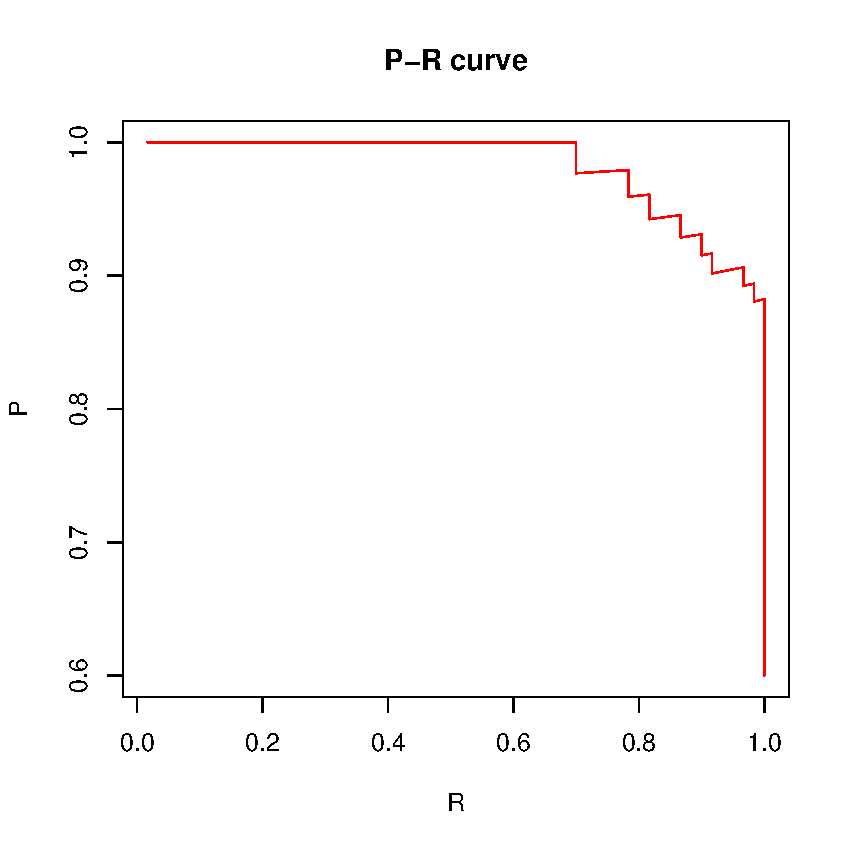
\includegraphics[width=0.65\textwidth]{P-R.pdf}
	\caption{P-R 曲线示例}
	\label{pr}
\end{figure}


\subsection{ROC 曲线与 AUC}
在二分类问题中, 还有两个常用的评价指标, 由于我们主要关注正样本, 因此引入了两个指标: TPR 和 FPR.

所谓 TPR(True Positive Rate), 即“真正例率”, 也称为敏感性(Sensitivity), 其实就是查全率, 即真正的所有正类(TP + FN)中, 确实被我们预测为了正类的(TP)占的比例, 或者说“正例的覆盖率”
\begin{equation}
TPR = \frac{TP}{TP + FN}
\end{equation}

所谓 FPR(False Positive Rate), 即“假正例率”, 是指真正的所有负类(FP + TN)中, 被我们错误的预测为了正类的(FP)占的比例
\begin{equation}
FPR = \frac{FP}{FP + TN}
\end{equation}

我们自然希望 TPR 能尽量地大, 而 FPR 尽量地小, 但这也是很难达到的.

同“P-R”曲线一样, 有的模型如 Logistic 回归可以返回样本属于正类的概率, 这样可以设定不同的阈值来对样本进行归类, 这样可以计算出一系列的 TPR 值和 FPR 值. 比如设定阈值为 0 时, 那么所有的样本都会被预测为正类, 此时 TPR = 1, 而 FPR = 1, 随着阈值逐渐增大, 被预测为正类的样本数逐渐减少,  TPR 和 FPR 也会各自减小, 当阈值增大至 1 时, 没有样本被预测为正类, 此时 TPR = 0, FPR = 0. 以 TPR 为纵轴、FPR 为横轴也可画出一条曲线, 称为 ROC 曲线, 其全称是“受试者工作特征”(Receiver Operating Characteristic)曲线, 如下图\ref{roc}所示.
\begin{figure}[!htb]
	\centering
	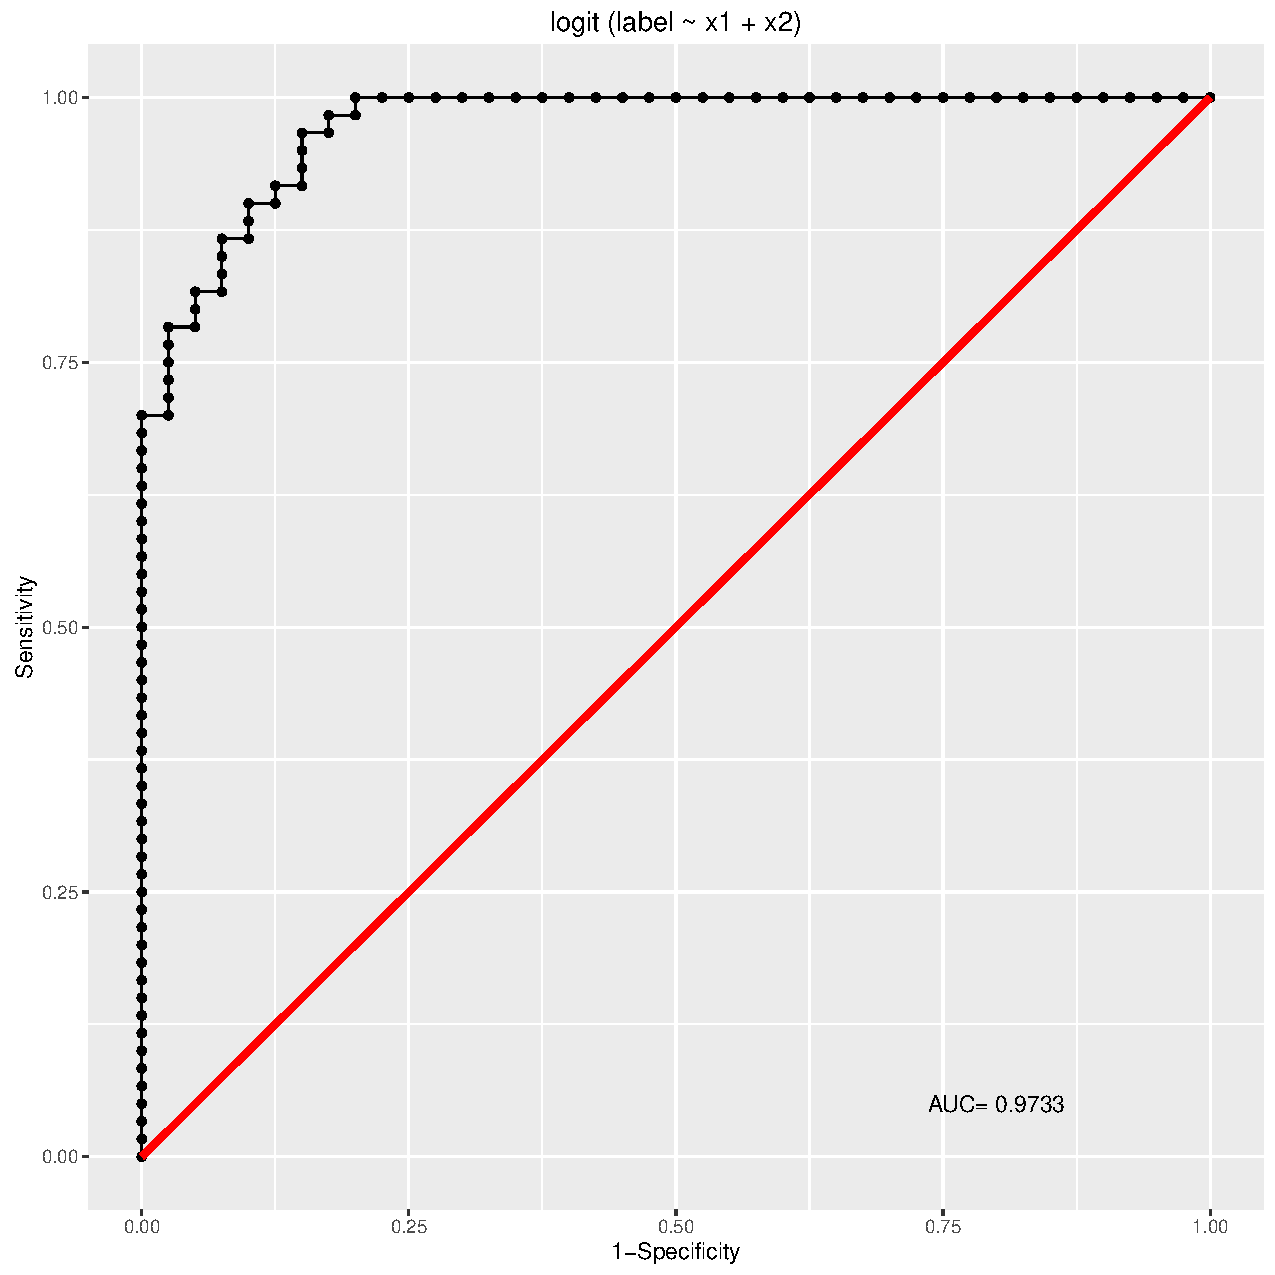
\includegraphics[width=0.65\textwidth]{ROC.pdf}
	\caption{ROC 曲线示例}
	\label{roc}
\end{figure}

TPR 和 FPR 存在同方向变化的关系, 而我们一般希望提升 TPR, 减小 FPR, 所以通常还是很难达到的.

当模型预测效果较好时, ROC 曲线会凸向左上角的顶点, 即模型的 TPR 值大, 且 FPR 值小, 模型越好, 其 ROC 曲线越远离对角线.

ROC 曲线下的面积是评价模型的一个合理标准, 记作 AUC(Area Under ROC Curve), AUC 越大模型效果一般越好.

这里提一下, 由混淆矩阵的那 4 个量(TP, FP, FN, TN)可以计算出很多指标(可参考 \url{https://en.wikipedia.org/wiki/Sensitivity_and_specificity} 或 \url{https://en.wikipedia.org/wiki/Confusion_matrix}), 这里就不详述了, 比如“真负例率”, 也记为 specificity(SPC), 即
\begin{equation}
SPC = \frac{TN}{TN + FP} = 1 - FPR
\end{equation}

这样的话, ROC 曲线的横轴也可表示为 1 - SPC. 其他就不多说了.


\section{总结}
\subsection{参考资料}
\begin{enumerate}[(1)]
\item 知乎: \url{https://www.zhihu.com/collection/45422299}, 魏晋的回答, 理清了一些关系, 虽然是借着生成模型与判别模型的区别回答的.

\item 博客: \url{http://www.flickering.cn/%E6%95%B0%E5%AD%A6%E4%B9%8B%E7%BE%8E/2014/06/lda%E6%95%B0%E5%AD%A6%E5%85%AB%E5%8D%A6mcmc-%E5%92%8C-gibbs-sampling/}, 理论介绍的更为详细一些.


\end{enumerate}





\begin{thebibliography}{4}
  \bibitem{1} 李荣华.\emph{偏微分方程数值解法}.高等教育出版社(2010) 
  \bibitem{2} Zhilin Li,Zhonghua Qiao,Tao Tang.\emph{Numerical Solutions of Partial Differential Equations-An Introduction to Finite Difference and Finite Element Methods}.(2011)
  \bibitem{3} 孙志忠.\emph{偏微分方程数值解法}.科学出版社(2011)

\end{thebibliography}

\newpage

\section*{附录}








\end{document}